\documentclass[10pt,answers]{exam}
\usepackage{mathtools,amsmath,amssymb,amsthm,mathrsfs}
\usepackage{pgfplots}
\usepackage{pgfplotstable}
\usepackage[multidot]{grffile}
\usepackage{pgf,tikz}
\usetikzlibrary{shapes,backgrounds,positioning,matrix,decorations}

\usepackage{siunitx}
\usepackage{ifxetex,ifluatex}
\title{Solution to Homework 1}
\author{Dilawar Singh}
\date{\today}
\usepackage{pgfplots}
\usepackage{booktabs,longtable}
\usepackage{subfig}

\begin{document}
\maketitle

\begin{questions}

\question{Coding}

Consider a horse race where the probabilities of winning are given by
negative powers of 2 (1/2, 1/32, etc.). Suppose the lowest possible
probability for any horse is \(2^{-m}\), and that there are \(n_i\)
horses in each probability class \(2^{-i}\).

\begin{parts}
    
\part[2] What equation must the \(n_i\) satisfy?

\begin{solution}
    Total probability (probability of all events) must adds up
    to 1 i.e., \(\sum_i n_i2^{-i} = 1\).
\end{solution}

\part[3] Give 3 possible sets of \(\{n_i\}\) for an 8 horse race (other than
  the uniform case).

\begin{solution}
\begin{longtable}[]{@{}llllll@{}}
  \toprule
  \(1/2\) & \(1/4\) & \(1/8\) & \(1/16\) & \(1/32\) &
  Entropy\tabularnewline
  \midrule
  \endhead
  0 & 0 & 8 & 0 & 0 & 3.0\tabularnewline
  0 & 1 & 5 & 2 & 0 & 2.875\tabularnewline
  0 & 2 & 2 & 4 & 0 & 2.75\tabularnewline
  0 & 2 & 3 & 1 & 2 & 2.6875\tabularnewline
  0 & 3 & 0 & 3 & 2 & 2.5625\tabularnewline
  0 & 3 & 1 & 0 & 4 & 2.5\tabularnewline
  1 & 0 & 1 & 6 & 0 & 2.375\tabularnewline
  1 & 0 & 2 & 3 & 2 & 2.3125\tabularnewline
  1 & 0 & 3 & 0 & 4 & 2.25\tabularnewline
  1 & 1 & 0 & 2 & 4 & 2.125\tabularnewline
  \bottomrule
  \caption{Distribution of horses into probability classes.}\label{tab:1}
\end{longtable}
\end{solution}

\part[3] Using the entropy concept, calculate the expected codeword length for
  each set.
  \begin{solution}
      See the table \ref{tab:1}.
  \end{solution}
\part[6] For each set, present an efficient binary coding scheme that achieves
  optimality.
  \begin{solution}
  \end{solution}
\end{parts}

Script \texttt{./problem1.py} generates some solutions (probably all possible)
to this problem. They are listed below.

Code are not given. Your code must be decodable and its entropy should be near
or equal to calculated entropy given in table above.


\question{[CT 2.13] Coin weighing.}

Suppose one has n coins, among which there may or may not be one
counterfeit coin. If there is a counterfiet coin, it may be either
heavier or lighter than the other coins. The coins are to be weighed by
a balance.

\begin{parts}
    \part[5]
    Find an upper bound on the number of coins n so that k weighing will
    find the counterfeit coin (if any) and correctly declare it to be
    heavier or lighter.
    \begin{solution}
        Lets not do any guess work! We draw \(k\) coins and weigh
        them with another \(k\) coins.

        The probability that counterfeit coins is in selected k coins is
        \(p(k)\). It is easy to show that \(p(k) = \frac{k}{12}\). We have three
        partitions of size $k$, $k$, and $12-k$.

        We can only weigh partition of size $k$ with other partition of size $k$.
        Weighing $k$ coins with $12-k$ coins is pointless (proof?). If counterfeit
        is in any of $k$-size partitions, then we reduce the state space to $2k$;
        otherwise the counterfeit coin is in rest of the $12-k$ coins (reduce the
        state space to $12-k$).

        With probability \(p(k)\) (that counterfeit coin is in selected $k$
        coins), we reduce the state space by $2k$ (or to $12-2k$); and with
        probability \(1-p(k)\) by ($12-2k$) (or by $2k$) i.e. average reduction is
        \(w(k)=p(k)(12-2k)+(1-p(k))(2k)\). What value of \(k\) maximize this
        function? It is maximum as $k=4$, and $k=5$.

        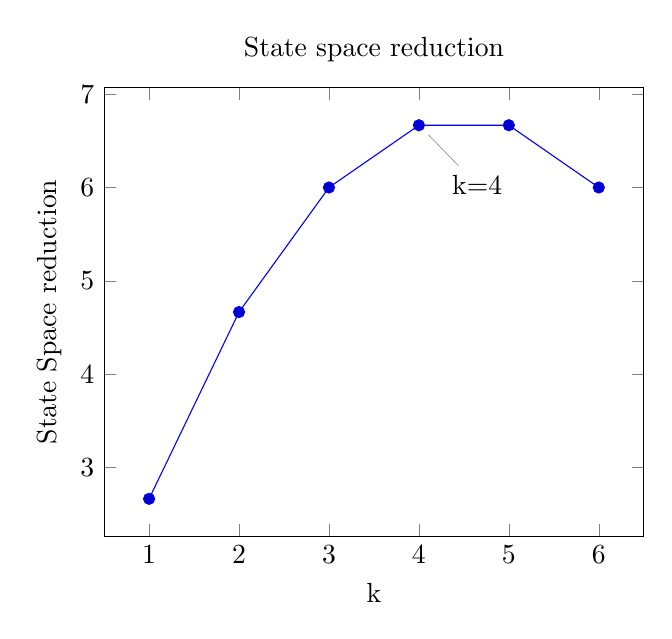
\begin{tikzpicture}[scale=1]
            \begin{axis}[ xlabel=k, ylabel=State Space reduction, domain=1:6
                , samples=6
                , title = {State space reduction}
                ]
                \addplot+ [color=blue,] plot { x/12 * (12-2*x) + (1 - x/12) * 2*x };
                \node[pin=-60:{k=4}] at (axis cs:4,6.67) { };
            \end{axis}
        \end{tikzpicture}

        You can weigh 4 or 5 coins with another equal number of coins. 

    \end{solution}



    \part[5] Suppose you have k = 3 weighings and 12 coins. How many coins must you
    weigh against each other in the first round?

    \begin{solution}
        
    Now lets assume the genralised case of N coins, if we weigh k coins with
    each other, \(w(k) = 3k - \frac{4k^2}{N}\). Its maximum when \(k =
    \frac{3N}{8}\).  Let's assume the worst case that the counterfiet coins
    always end up in the 2k coins which we weigh against each other. At each
    weigh, we pick the optimal number of coins (\(\frac{3N}{8}\)) and reduce the
    state space by 2k ( \(\frac{3N}{4}\)). First step we have \(N\) coins, after
    one weigh we have \(3N/2\) coins, after second weigh we have
    \(\frac{3}{4}\frac{3N}{4}\), and so on. After \(n\) weigh, we have
    \(\frac{3}{4}^n N\) coins. We stop when we are left with 2 coins. One more
    additional weigh, will tell which one is counterfiet.

    \(\frac{3}{4}^n N = 2 \implies n = \frac{\ln{2/N}}{\ln{3/4}} = 3.476 \ln{\frac{N}{2}}\).
    Therefore number of maximum weighings are \(3.467\ln{N/2}\). For N=12,
    the value is much higher than 3. Needless to say, this is not the most
    efficient strategy.

    \end{solution}

    \bonuspart[15] (Optional, and hard) Find the full strategy for the 12 coin case.
    \begin{solution}
        First we divide the coins into three equal parts and weigh one part with
        rest of two parts (2 weighing). This will tell us if the counterfiet
        coins is heavier or lighter; and also in which N/3 coins it is in.

        Once we have done that, we take the N/3 coins, again divide into 3
        parts, do one weighing of 1 part with another and we can declare the
        part the cointerfeit coin is in. Therefore, starting with N/3, and at
        each step dividing the states into 3 parts, after (k-2) weighing, we
        must figure out the coin. Therefore
        \(\frac{1}{3}^{k-2} \frac{N}{3} = 1 \implies k = 2 + 0.91 \ln \frac{N}{3}\).
        For N = 12, we have \(k = 3.26\); very near to optimal solution.

    \end{solution}

\end{parts}



\end{questions}

\end{document}
